% It is an example file showing how to use the 'sigkddExp.cls' 
% LaTeX2e document class file for submissions to sigkdd explorations.
% It is an example which *does* use the .bib file (from which the .bbl file
% is produced).
% REMEMBER HOWEVER: After having produced the .bbl file,
% and prior to final submission,
% you need to 'insert'  your .bbl file into your source .tex file so as to provide
% ONE 'self-contained' source file.
%
% Questions regarding SIGS should be sent to
% Adrienne Griscti ---> griscti@acm.org
%
% Questions/suggestions regarding the guidelines, .tex and .cls files, etc. to
% Gerald Murray ---> murray@acm.org
%

\documentclass{article}
\usepackage{cite}
\usepackage{amssymb}
\usepackage{amsmath}
\usepackage{amsfonts}
\usepackage{algorithm2e}
\usepackage{rotating}

\usepackage{tikz}
\usetikzlibrary{shapes,arrows}
\usepackage{bm,times}
\usetikzlibrary{shapes.geometric, arrows}

\tikzstyle{sensor}=[draw, text centered, minimum height=2.5em]
\tikzstyle{ann} = [minimum width=8em, text centered]
\tikzstyle{data} = [draw, rounded corners, minimum width=3cm, minimum height=1cm, text centered, text width=4cm, draw=black]
\tikzstyle{wa} = [draw, rounded corners, minimum width=3cm, minimum height=1cm, text centered, text width=3cm, draw=black]
\tikzstyle{sc} = [sensor, text width=13em, 
    minimum height=10em, rounded corners]
\def\blockdist{1.5}
\def\edgedist{2.5}
\pgfdeclarelayer{background}
\pgfdeclarelayer{foreground}
\pgfsetlayers{background,main,foreground}



\begin{document}

%
% --- Author Metadata here ---
% -- Can be completely blank or contain 'commented' information like this...
%\conferenceinfo{WOODSTOCK}{'97 El Paso, Texas USA} % If you happen to know the conference location etc.
%\CopyrightYear{2001} % Allows a non-default  copyright year  to be 'entered' - IF NEED BE.
%\crdata{0-12345-67-8/90/01}  % Allows non-default copyright data to be 'entered' - IF NEED BE.
% --- End of author Metadata ---

\title{Exact and Online Distributed Bootstraps}
\author{William High}
\date{\today}
\maketitle

\begin{abstract}

This paper presents an exact, nonparametric distributed bootstrap method for
bounded data and an online variant that may be used on unbounded streaming
data. The exact distributed bootstrap procedure is to split a finite data set
among nodes of a distributed computer system; asynchronously execute standard,
non-parametric bootstrap resampling of a (possibly multivariate) statistic on
each node; output the statistic and associated weights from each bootstrap
iteration on each node to a master node; and on the master node aggregate the
statistic in each bootstrap bucket. The final product is a bootstrap sample
distribution of the statistic. For exactness, the method requires an exact
update rule for the statistic under study on the master node. I demonstrate
this with a canonical weighted mean and weighted standard deviation update
rule example. The method is still viable and handy but becomes approximate
when the update rule is itself not exact.  I explore an online variant of the
exact distributed bootstrap, which permits real-time updates of the bootstrap
distribution on each node and on the master node.

\end{abstract}

\section{Introduction}

The nonparametric bootstrap \cite{bib:efron} is incredibly useful for
empirically estimating sampling distributions where closed form sample summary
statistics may be inaccurate or unavailable.  Given a data set of size $n$,
the method is to randomly sample $n$ data points with replacement in $r$ total
iterations, where $r \gtrsim 200$, and execute an analysis pipeline to produce
a statistic at each iteration. The histogram of the statistic from each
iteration is an estimate of the sample distribution of that statistic. For
example, the mean of the bootstrap distribution is an estimate of the sample
mean; the standard deviation is an estimate of the standard error on the mean;
confidence intervals are computed on the histograms directly; and covariance
on a multivariate statistic can also be computed on the joint bootstrap
distribution directly.

The online bootstrap sketched by \cite{bib:onlineboot} is a variant of the
bootstrap that processes one data point at a time.  The essential observations
are that a single given data point is sampled in $n$ trials with probability
$1/n$ per trial in a single bootstrap iteration, so the number of samples for
each data point is distributed as $Binomial(n,1/n)$; and for moderate to large
$n$, $Binomial(n,1/n)$ converges to $Poisson(1)$.  Turning this logic around,
given a single data point in a given bootstrap iteration, using an importance
weight $w$ drawn randomly from $Poisson(1)$ emulates the bootstrap resampling.
If the data point already has an importance weight $w^{\prime}$, then the
final online bootstrap resample importance weight is $W = w^{\prime}w$.

The Bag of Little Bootstraps is a variant of the bootstrap that can be run on distributed 
data \cite{bib:blb}. In this setting, the larger data set of size $n$ is randomly distributed or ``split''
across $s$ nodes, and each split has size $b$.  

These authors had in mind
big data that is split across nodes, such as on the Hadoop Filesystem. The BLB
procedure is to run the bootstrap on each node that can locally access,
compute a statistic (e.g.\ the mean, confidence interval) on each bootstrap
distribution separately, then collect the statistic from each node and average
to produce a global statistic.

As stated, the method requires that you know the size of each data split and
the total size of the data set, and that you can compute and store a reservoir
of resample indexes in memory. It also makes the interesting choice of
aggregating up the bootstrap distribution to a summary statistic on each node,
and then average each summary statistic, which speeds up the algorithm but
doesn't allow for the mining of additional bootstrap distribution summary
statistics after the fact.

\section{The Algorithms}

\subsection{Exact Distributed Bootstrap}

Given that $r$ is typically chosen to be of order $10^2$ to $10^4$ or so, it's
reasonable to aggregate and persist $r$ bootstrap buckets on a node or set of
nodes using an online bootstrap bucket update rule.

The inner bootstraps require an online update rule that respects importance
weights. The outer bootstrap aggregator requires a different

Algorithm \ref{algo:exact} outlines the OBLB idea.

\begin{algorithm}
\caption{Exact batch distributed bootstrap}
\label{algo:exact}
\DontPrintSemicolon
\SetKwFunction{InnerBatchUpdate}{InnerBatchUpdate}
\SetKwFunction{MasterBatchUpdate}{MasterBatchUpdate}
\SetKwFunction{MultinomialRandom}{MultinomialRandom}
\SetKwInOut{Input}{Input}
\SetKwInOut{Output}{Output}
\Input{Bounded data-weight tuples, $\{(X_1,w^{\prime}_1), (X_2,w^{\prime}_2), ..., (X_n,w^{\prime}_n)\}$
    \\
    Number of bootstrap realizations, $r$
    \\
    Number of nodes, $s$
    \\
    Size of data subset that is local to node $j\in \{1,2, ..., s\}$, $b_j$ 
}
\Output{Estimator value in each bootstrap realization, $\hat\theta_{k}\;\forall \; k\in \{1, 2, ...., r\}$}
\For{$j \gets 1$ \KwTo $s$}{
    Retrieve local set of data-weight tuples, $(\boldsymbol{X}_j,\boldsymbol{w}_j)$\;
    Compute $b_j$\;
    \For{$k \gets 1$ \KwTo $r$}{
        $\boldsymbol{W} \gets \boldsymbol{w}^{\prime}_j \cdot \MultinomialRandom(b_j,\boldsymbol{1}_{b_j}/b_j)$\;
        $(\hat\theta_{jk}, w_{jk}) \gets \InnerBatchUpdate(\boldsymbol{X}_j, \boldsymbol{W})$\;
    }
}
\For{$k \gets 1$ \KwTo $r$}{
    $\hat\theta_{k} \gets \MasterBatchUpdate(\hat\theta_{jk}, w_{jk})$\;
}
\Return $\boldsymbol{\hat\theta}$
\end{algorithm}


\subsection{Online Distributed Bootstrap}

\begin{algorithm}
\caption{Online distributed bootstrap}
\label{algo:online}
\DontPrintSemicolon
\SetKwFunction{InnerOnlineUpdate}{InnerOnlineUpdate}
\SetKwFunction{MasterOnlineUpdate}{MasterOnlineUpdate}
\SetKwFunction{PoissonRandom}{PoissonRandom}
\SetKwFunction{UpdateMaster}{UpdateMaster}
\SetKwInOut{Input}{Input}
\SetKwInOut{Output}{Output}
\Begin{
    \Input{Unbounded data-weight tuples, $\{(X_1,w^{\prime}_1), (X_2,w^{\prime}_2), ...\}$
        \\
        Number of bootstrap realizations, $r$
        \\
        Number of nodes, $s$
        \\
        Online estimator update rule OnlineUpdate
    }
    \Output{Estimator value in each bootstrap bucket, $\hat\theta_{k}\;\forall \; k\in \{1, 2, ...., r\}$}
    \For{$k \gets 1$ \KwTo $r$}{
      $w_{k} \gets 0$\;
      $\hat\theta_{k} \gets 0$\;
      \For{$k \gets 1$ to $r$}{
        $w_{jk} \gets 0$\;
        $\hat\theta_{jk} \gets 0$\;
      }
    }
    \For{$i \gets 1$ to $\infty$}{
      Assign tuple $(X_i,w^{\prime}_i)$ to node $j \in \{1, 2, ..., s\}$\;
      \For{$k \gets 1$ to $r$}{
        $W \gets w^{\prime}_i \times \PoissonRandom(\lambda = 1)$\;
        $(\hat\theta_{jk}, w_{jk}) \gets \InnerOnlineUpdate(\hat\theta_{jk}, w_{jk}, X_i, W)$\;
      }
      \If{$\UpdateMaster()$} {
        \For{$k \gets 1$ to $r$}{
          $(\hat\theta_{k}, w_{k}) \gets \MasterOnlineUpdate(\hat\theta_{k}, w_{k},\hat\theta_{jk}, w_{jk})$\;
          $w_{jk} \gets 0$
          \\
          $\hat\theta_{jk} \gets 0$
        }
      }
    }
}
\end{algorithm}

A flowchart is shown in Figure \ref{oblbflowchart}.

\begin{sidewaysfigure}[tbp]
\centering
\label{oblbflowchart}
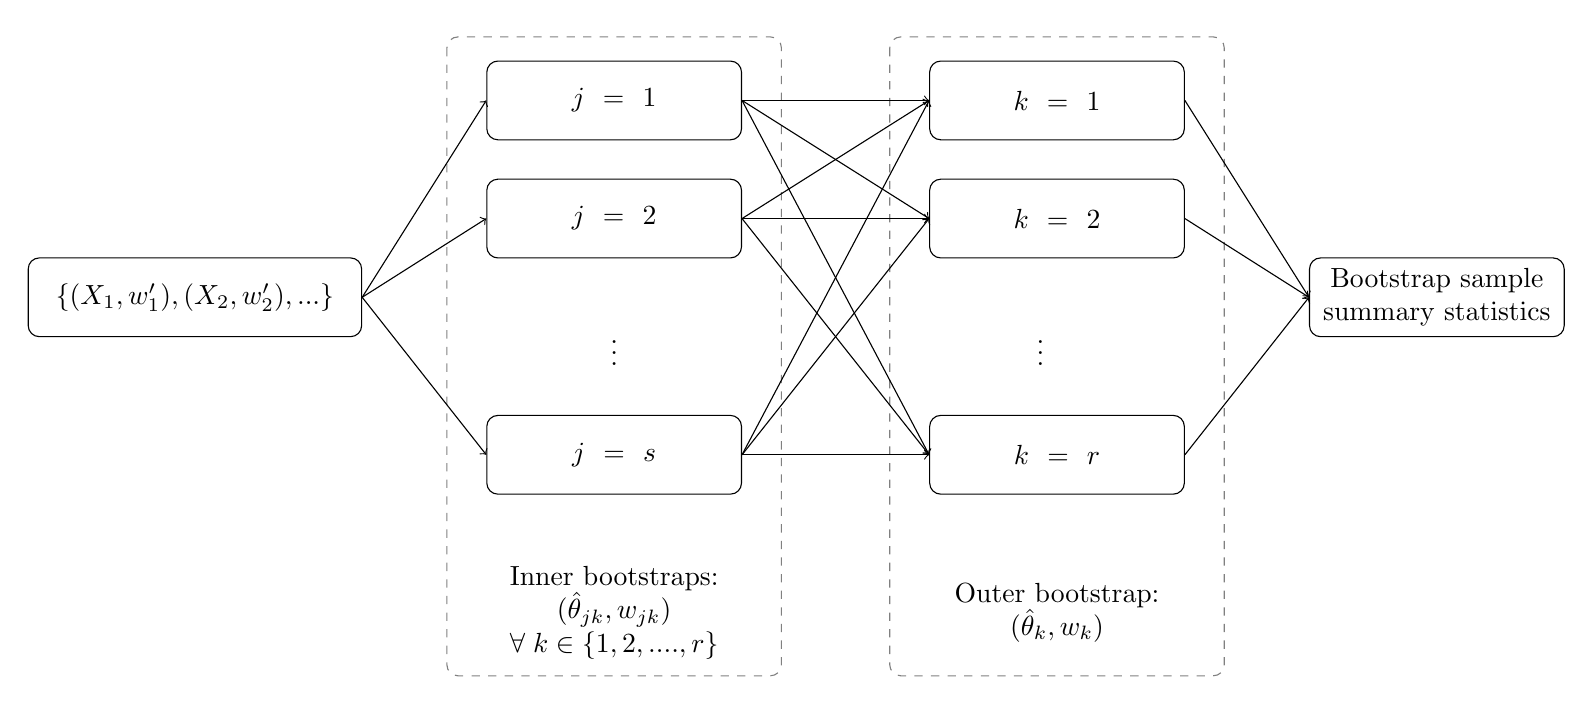
\begin{tikzpicture}
    \node (data) [data]  {$\{(X_1,w^{\prime}_1),(X_2,w^{\prime}_2),...\}$};

%    \path (data.east)+(3.2,2.5) node (innerboot1) [wa] {$(\hat\theta_{jk},w_{jk})$, $j=1$, $\forall\,k\in\{1,2,...,r\}$};
    \path (data.east)+(3.2,2.5) node (innerboot1) [wa] {$j=1$};
    \path (data.east)+(3.2,1) node (innerboot2)[wa] {$j=2$};
    \path (data.east)+(3.2,-0.6) node (dots1)[ann] {$\vdots$}; 
    \path (data.east)+(3.2,-2) node (innerboot3)[wa] {$j=s$}; 
    \path (innerboot3.south) +(0,-\blockdist) node (asrs)[align=center] {Inner bootstraps:\\$(\hat\theta_{jk},w_{jk})$\\$\forall \; k\in \{1, 2, ...., r\}$};
    
    \begin{pgfonlayer}{background}
        \path (innerboot1.west |- innerboot1.north)+(-0.5,0.3) node (a) {};
        \path (innerboot3.south -| innerboot3.east)+(+0.5,-0.3) node (b) {};
        \path (innerboot3.east |- asrs.east)+(+0.5,-0.8) node (c) {};
        \path[rounded corners, draw=black!50, dashed]
            (a) rectangle (c);           
        \path (innerboot3.north west)+(-0.2,0.2) node (a) {};
    \end{pgfonlayer}

    \path (innerboot1.east)+(4,0) node (outerboot1) [wa] {$k=1$};
    \path (innerboot2.east)+(4,0) node (outerboot2) [wa] {$k=2$};
    \path (dots1.east)+(4,0) node (dots2)[ann] {$\vdots$}; 
    \path (innerboot3.east)+(4,0) node (outerboot3)[wa] {$k=r$};    
    \path (outerboot3.south) +(0,-\blockdist) node (asrs)[align=center] {Outer bootstrap:\\$(\hat\theta_{k},w_{k})$};
    
    \begin{pgfonlayer}{background}
        \path (outerboot1.west |- outerboot1.north)+(-0.5,0.3) node (a) {};
        \path (outerboot3.south -| outerboot3.east)+(+0.5,-0.3) node (b) {};
        \path (outerboot3.east |- asrs.east)+(+0.5,-0.8) node (c) {};
        \path[rounded corners, draw=black!50, dashed]
            (a) rectangle (c);           
        \path (outerboot3.north west)+(-0.2,0.2) node (a) {};
    \end{pgfonlayer}

    \path (outerboot2.east)+(3.2,-1) node (masterboot) [wa]  {Bootstrap sample\\summary statistics};

    \foreach \x in {1,2,3} 
    {
        \path [draw, ->] (data.east) -- node [above] {} (innerboot\x.west);
    }

    \foreach \x in {1,2,3} 
    {
        \foreach \y in {1,2,3} 
        { 
            \path [draw, ->] (innerboot\y.east) -- node [above] {} (outerboot\x.west);
        }
    }
    
    \foreach \x in {1,2,3} 
    {
        \path [draw, ->] (outerboot\x.east) -- node [above] {} (masterboot.west);
    }



                
\end{tikzpicture}
\caption{Schematic representation of the algorithm.}
\end{sidewaysfigure}


\section{Comparison}

Table \ref{bootcomp}

\begin{table}[h]
\caption{Properties of different bootstrap methods.}
\label{bootcomp}
\begin{tabular}{lllll}
\hline
\hline
Property/requirement & Bootstrap & OB & BLB & OBLB \\
\hline
Online & No & Yes & No & Yes \\ 
Distributed & No & No & Yes &  Yes \\ 
Resampling index precompute & Yes & No & Yes & No \\ 
Req.\ bounded data & Yes & No & Yes & No \\ 
Req.\ known bound & Yes & No & Yes & No \\ 
Maintains bootstrap histogram & Yes & Yes & No & Yes \\
\hline
\hline
\end{tabular}
\end{table}


\section{Simulations}

\subsection{Sample Mean}

Algorithm \ref{onlineupdate} is a canonical example of an online update rule: the weighted mean. 
The weighted mean can be computed on streaming data by maintaining the mean and the aggregate
weight. The unweighted mean is the limiting case where the data weights are all one.

\begin{algorithm}
\caption{OnlineUpdate example: streaming weighted mean}
\label{onlineupdate}
\DontPrintSemicolon
\SetKwInOut{Input}{Input}
\SetKwInOut{Output}{Output}
\Input{Current mean $\theta_0$
  \\
  Aggregate weight of current mean $w_0$ 
  \\
  New data $X$
  \\
  Weight of new data $W$
}
\Output{Updated mean $\theta_1$
    \\
    Aggregate weight of updated mean $w_1$
}
$\theta_1 \gets (w_0\theta_0 + WX)/(w_0 + W)$
\\
$w_1 \gets w_0 + W$ 
\\
\Return $(\theta_1, w_1)$
\end{algorithm}

If both OnlineUpdate and OnlineMasterUpdate use the online weighted mean algorithm, 
then OBLB is equivalent to the traditional, serial, nonparametric 
bootstrap of the weighted mean, up to numerical errors at the machine precision
level.

\subsection{Online Logistic Regression Trainer}


\section{Conclusions}





\bibliography{online_blb}{}
\bibliographystyle{plain}

\end{document}
